\documentclass[border=10pt]{standalone}
\usepackage{pgfplots}
\pgfplotsset{compat=1.18}
\begin{document}
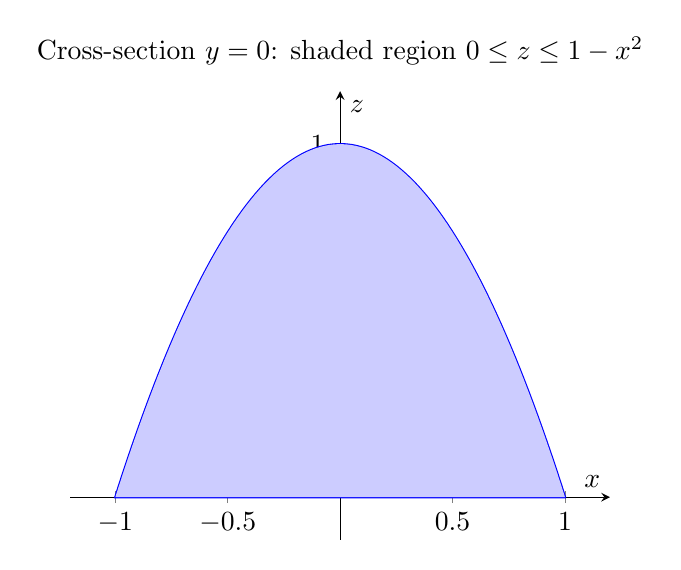
\begin{tikzpicture}
\begin{axis}[
    axis lines = middle,
    xlabel={$x$}, ylabel={$z$},
    xmin=-1.2, xmax=1.2, ymin=-0.12, ymax=1.15,
    domain=-1:1, samples=100,
    title={Cross-section $y=0$: shaded region $0 \le z \le 1-x^2$},
]
\addplot[thick, color=blue] {1-x^2} \closedcycle;
\addplot[color=blue!25] coordinates {(0,0)} \closedcycle;
\addplot[domain=-1:1, samples=100, draw=none, fill=blue!20]
    {1-x^2} \closedcycle;
\end{axis}
\end{tikzpicture}
\end{document}